% packages
\documentclass[letterpaper, 10pt, conference]{article}
%\documentclass[iros]{IEEEtran}

\usepackage{graphicx}
\usepackage{cite}
\usepackage{soul,color}
\usepackage{amssymb}
\usepackage{amsmath}
\usepackage{subcaption}

\usepackage[margin=1in]{geometry}  % Adjust margins as needed
\usepackage{lipsum}  % For generating placeholder text, remove in your actual paper


\begin{document}

%GenTLEBot
\title{Legibot: Legible Motions for Service Robots} % \\ \large by Motion Prediction based on Visual Cues}
\author{Javad Amirian} %, Mouad Abrini, Mohamed Chetouani}
\maketitle

\begin{abstract}
With the prevalence of social robots in various environments and applications, there is an increasing need for these robots to exhibit socially-compliant behaviors.
Legible motion, characterized by the ability of a robot to clearly and quickly convey intentions and goals to the individuals in its vicinity, holds significant importance in this context.
%
%In this paper, we introduce a pioneering framework for assessing the legibility of robot motion.
%Our approach leverages optical flow-based visual input to simulate how a human observer perceives a robot's actions.
%
In this paper, we introduce a novel approach to incorporate legibility into local motion planning for mobile robots.
This can enable robots to generate legible motions in real-time and dynamic environments.
%
To demonstrate the effectiveness of our proposed methodology,
we conducted real-world experiments involving the Pepper robot and simulated scenarios featuring mobile robots in a restaurant environment with multiple human occupants.
\end{abstract}

%\setcounter{section}{-1} % Set section counter to -1
\section{TODOs}

\begin{itemize}
    \item Study the impact of the robot's HEADING (Gaze) vs Direction of Motion when perceived by an observer
    
    \item Generate Trajectories
    
    \item Submit Ethics Approval
\end{itemize}



\section{Introduction}
% ================ General Intro: Social Robots ================
~
%Robots are not limited to factories and fabrication lines anymore and they are becoming more and more of a Must for service-oriented tasks, such as in hospitals, hotels, restaurants, and so on.
%
%This means they should understand, and respect the -unwritten social rules that define how people expect other agents to behave around them.
%This is what is called social-compliant behaviors and Francis et al [REF] pointed out there are eight different sets of principles for a robot to become socially compliant, including safety, politeness, legibility, and so on.
%Even though these axes are not necessarily orthogonal which means improving on one aspect can impact other aspects, either negatively or positively.
%
%Among those, legibility is a less-developed concern in robots and has a long way to go.
%legible motion, is characterized by the ability of a robot to clearly and quickly convey intentions and goals to the individuals in its vicinity holds significant importance in this context.
%
Robotic systems have transcended their traditional roles in factories and manufacturing lines, expanding into various service-oriented domains, including healthcare, hospitality, and food service.
As robots increasingly share spaces with humans, it becomes imperative for them to comprehend and adhere to the implicit social norms that govern human interaction.
This imperative gives rise to the concept of social-compliant behaviors, wherein robots are expected to exhibit behaviors that align with human expectations.
Francis et al. \cite{francis2023principles} have identified eight distinct sets of principles that collectively define social compliance for robots, encompassing aspects such as safety, politeness, and legibility.
Notably, these dimensions are not mutually exclusive; improvements in one dimension can influence others, either positively or negatively.

% ================ Intro: Legibility ================
Among these dimensions, legibility remains an underdeveloped aspect in the field of robotics and presents substantial room for advancement.
Legibility in robotic motion refers to the robot's capacity to clearly and swiftly communicate its intentions and objectives to individuals in its vicinity.
In the context of human-robot interaction, achieving legible motion is of paramount significance, as it enhances user understanding, trust, and overall user experience.
%
It might sometimes be simply as the agent's effort to exaggerate its action to make sure the opponent is aware of its decision, which can be critical in human-robot tasks that require tight collaboration between the two parties.
But, also it can appear in more complex scenarios to respect the social rules in a certain space, and adapt to some acceptable behaviors in that context.

%\subsection{A Note from Cognitive Science}
%Human brains makes significant efforts in the prediction of the events around a person. This predictions happen in short-term and long-term ways, to help the person for making decision. One of such predictions is about moving objects.
%The brain processes moving objects, starting with the retina's photoreceptor cells that send signals via the optic nerve to the thalamus and the primary visual cortex (V1). Directionally selective neurons in V1 respond to movement.
%Information then travels to areas like MT and MST, enabling the brain to construct a mental representation of the moving object, including its location, speed, and direction. This representation guides eye and body movements for tracking and interaction.


%%%
%This concept was initially raised by Dragan et al. [REF] to distinguish predictable behavior from legible behavior.
%A https://www.overleaf.com/project/65169f082a77e596ef35ffccmain pitfall though is that the original framework does not introduce any notion of an observer agent in the environment.
%There have been a few steps in recent years to address this gap, including Taylor et al. [REF] who tried to take the field-of-view of an observer agent into account, and Nikolaidis et al. [REF] who tried to include viewpoint into the formula and also formulate the occlusion. 

%\subsection{Contributions}
%The concept of legibility in robot behavior was initially introduced by Dragan et al. \cite{dragan2013legibility} as a means to differentiate predictable behaviors from legible actions.
%One limitation of the original framework, however, is the absence of consideration for an observer agent within the environment.
%%
%In recent years, efforts have been made to address this gap in the literature.
%For instance, Nikolaidis et al. \cite{nikolaidis2016based} extended this work by introducing considerations of viewpoint and formulating solutions for handling occlusion scenarios.
%Taylor et al. [REF] sought to incorporate the perspective of an observer agent by taking their field of view into account.

%\hl{
%    We argue that the concept predictability that was put against legibility in the work of Dragan et al. \cite{dragan2013legibility} is more reminding us of efficiency rather than predictability.
%In other words, legibility is still a property that makes predictions simpler and more intuitive for the observers, while an efficient action is not necessarily legible, but not always intuitive for the observer either.
%The efficiency optimization process that is done by a machine does not make the outputs necessarily predictable or un-predictable.
%}

%In this work, we propose a new approach for computing the motion legibility.
%We go beyond the trajectory level computations and propose our method based on visual inputs and semantics information.
%For this we have studied a short-term motion prediction method and a long-term goal prediction algorithm in an effort to cover the gap in the existing research in addressing the visual inputs of a human observer for computing legibility.

% ================ Intro: Proposed Approach ================
\vspace{0.3cm}
\textbf{Contributions:} In this paper we propose a novel approach to incorporate legibility into local motion planning for mobile robots.
The proposed formulation enables robots to generate legible motions in real-time and dynamic environments.
These dynamic changes in the environment can appear in different forms, such as a moving target, finding about new irrelevant goals,
and also the set of observers that robot should be legible for.
...

\vspace{0.3cm}
%\noindent
\textbf{Structure:}
%In this paper, we explore whether it is possible to redefine legibility by shifting the focus from directly processing the robot's geometric trajectory to using visual inputs.
%This can help us to take one more step toward human-centric robot legible motions.
%Our approach leverages optical flow-based visual input to simulate how a human observer perceives a robot’s actions.
%
In the next section, we review the related work in the field \ref{sec:related_work}.
Then in section \ref{sec:method} we propose the aforementioned framework in detail,
and then in section \ref{sec:exp} we explain the experiments we conducted with simulated and real robots to demonstrate the effectiveness of our proposed methodology in a restaurant scenario.



%\section{Dynamic Legibility}

\begin{itemize}
    \item
    RQ1: How can legible motions be designed and implemented in HRC systems to enhance the transparency and understand robot actions and intentions?
%    \item
%    RQ2: What methods and technologies can be employed to enable the robot to take the user's perspective, and how does this enhance the efficiency and naturalness of collaborative interactions?
%    \item
%    RQ3: How can intention prediction in HRC be improved, and what are the key factors that influence the accuracy and speed of predicting user intentions?
\end{itemize}

Three assumptions for our problem:
\begin{itemize}
    \item
    We are developing a handover task between a robot and a human.
    \item
    The robot will track the human's head pose and gaze direction to compute the legibility of its motion.
    \item
    The generation of legible motions is done in real-time, and the robot should be able to generate legible motions for different scenarios.
\end{itemize}


Trajectory synthesis within dynamic environment:

\subsection{Background: Legibility}

\begin{equation}
    \mathbf{L}(\xi) = P(G^* |\xi_{S \rightarrow Q}) =
    \frac{\exp (-C(\xi_{S \rightarrow Q})) \int \exp( -C(\xi_{Q \rightarrow G}))}
         {\int \exp (-C(\xi_{S \rightarrow G}))}
\end{equation}

\subsection{Projection of the trajectory for a given observer}
Replace $C(\xi)$ with $T(C(\xi))$ where $T$ is the projection function from the observer's frame.

\subsection{Challenges}

\begin{itemize}
    \item \textbf{Moving Observer:} when the observer position moves from point $O_A$ to $O_B$, the robot's motion should adapt.
    should we re-calculate \ref{eq:legibility} from scratch? or can we use the previous calculation?\\
    \textit{Answer:} Now we should consider $T$ as a function of time, say $T^t$:

    \item \textbf{Prediction:} when we generate trajectory for time $t_0+dt$ in the future we need to have a prediction of the observer's position at that time.\\
    \textit{Answer:} It can be simply trajectory extrapolation, or we can also predict the intention of the user and use that to predict the observer's position.
    The prediction can be represented as a probability distribution (e.g. a Gaussian distribution) over the observer's position.
    Which means, the projected cost of $C(\xi_{Q \rightarrow G})$ will be a distribution over the cost ...
\end{itemize}

\subsection{Scenario:}
Here, we explain the scenario that we are working on ...



\section{Related Work}
In \cite{dragan2013legibility} Dragan et al. differentiate predictability and legibility, crucial for human-robot collaboration. They provide formal definitions, propose cost-based models for motion planning, and practically validate the contradiction between predictability and legibility in various characters.

Work \cite{taylor2022observeraware} addresses the problem of the limited field of view of observers. Their proposed algorithm models observer locations and perspectives, enhancing legibility by placing movements where easily be seen. The study shows that observer-aware legibility increases the duration of correct goal inferences, but non-targeted observers have lower performance when paths are personalized for others. The paper emphasizes the importance of considering an observer's environment for effective planning in scenarios like robot-assisted \textbf{restaurant} service. Also \cite{dragan2015effects} implemented a \textbf{coffee-shop} scenario. Participants collaborated with the robot to fulfill tea orders. The robot retrieved the appropriate cup, and participants selected ingredients based on the cup being retrieved.

In \cite{bronars2023_GLMM} the core idea is bringing end-to-end framework using conditional generative models to learn legible robot trajectories from multi-modal human demonstrations. 
%
Zheng et al. \cite{PAT2021IJSR} demonstrated a significant difference in how humans perceive and react to a robot based on its type. In their study, when comparing people's reactions to a semi-autonomous wheelchair with a human driver onboard to that of a humanoid robot, it became evident that there was a much higher level of respect for the wheelchair robot.

% TODO: to review
* Of course, we all are aware of how signaling lights are used in vehicles to show other people our intentions, there are also other modalities to communicate the intent can be used for example in IAN by Dugas et al. \cite{dugas2020_IAN} a Pepper robot uses hand gestures and nudges to communicate with the people around it and ask them to clear the way. 

* \cite{fukuchi2009focus}

\section{Background}
%! Author = javad
%! Date = 04/01/2024

\subsection{Legibility Score}

The original formula for motion legibility (by Dragan et al. \cite{dragan2013legibility}) for an observed trajectory $\xi$ \cite{dragan2013legibility} is as follows:

\begin{equation}
    \label{eq_dragan9}
    \text { legibility }(\xi)=\frac{\int P\left(G^* \mid \xi_{S \rightarrow \xi(t)}\right) f(t) d t}{\int f(t) d t}
\end{equation}

\noindent
This equation assumes $P\left(G \mid \xi_{S \rightarrow \xi(t)}\right)$ is the way an observer distributes probabilities to potential goals of the robot, with $G^*$ being the true goal of the robot, and $f(t)$ to be a descending function like $f(t)=T-t$ which assigns higher weights to the initial parts of the trajectory, justifying the fact that a legible motion should minimize the ambiguity as soon as possible for the observers.

To compute Eq. (\ref{eq_dragan9}), they use the Bayse' rule and rewrite $P\left(G^* \mid \xi_{S \rightarrow \xi(t)}\right)$ as below:

\begin{equation}
    \label{eq_dragan8}
    P\left(G \mid \xi_{S \rightarrow Q}\right) \propto \frac{\exp \left(-C\left(\xi_{S \rightarrow Q}\right)-C\left(\xi_{Q \rightarrow G}^*\right)\right)}{\exp \left(-C\left(\xi_{S \rightarrow G}^*\right)\right)} P(G)
\end{equation}

with $P(G)$ being a prior distribution of the potential goals and $C(\xi)$ being a cost function for an observed trajectory $\xi$ or an optimal trajectory $\xi^*$. In the original work of Dragan et al. \cite{dragan2013legibility} however, this is considered as a Euclidean distance between the initial and the goal point for the latter, which makes it too simplistic, i.e. a real human might use his own knowledge and reasoning for predicting the robot's goal based what they observe and making this simple assumption is not always aligned with human actualities.


% \begin{figure}
%     \centering
%     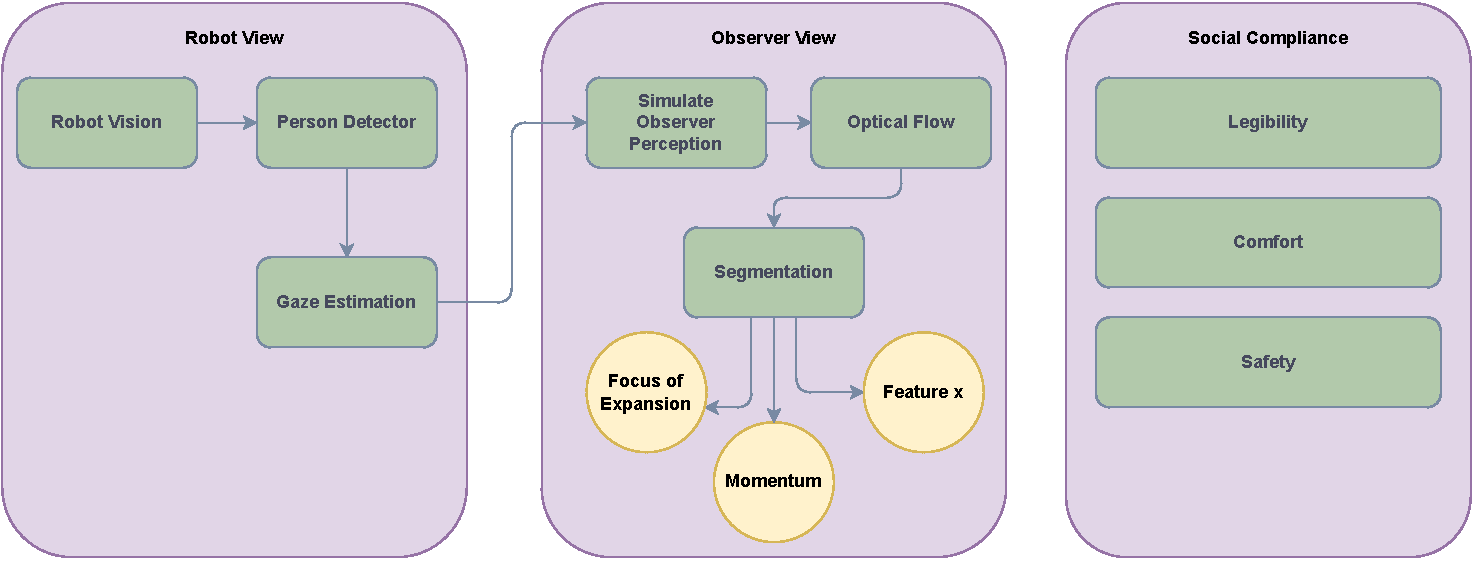
\includegraphics[width=0.8\textwidth]{figs/Legibot-fig1.pdf}
%     \caption{Overview}
%     \label{fig:enter-label}
% \end{figure}

\usepackage{latexsymb}

%    \section{Background}
%In this paper, we explore the question of whether it is possible to redefine legibility
%by shifting the focus from directly processing the robot's geometric trajectory to using visual inputs.
%This can help us to take one more step toward human-centric robot legible motions.

    %%%%%%%%% Copy from docs/iros2024/sections/intro.tex %%%%%%%%%


%\subsection{A Note from Cognitive Science}
%Human brains makes significant efforts in the prediction of the events around a person.
%This predictions happen in short-term and long-term ways, to help the person for making decision.
%One of such predictions is about moving objects.
%The brain processes moving objects, starting with the retina's photoreceptor cells that send signals via the optic nerve
% to the thalamus and the primary visual cortex (V1). Directionally selective neurons in V1 respond to movement.
%%
%Information then travels to areas like MT and MST, enabling the brain to construct a mental representation of the moving object,
% including its location, speed, and direction. This representation guides eye and body movements for tracking and interaction.


\section{Proposed Contributions:}
%    \noindent
%    \subsection{Modeling Visual Perceptions}
%
%    The concept of legibility against predictability of robot behavior was initially introduced by Dragan et al. \cite{dragan2013legibility}.
%    Even though in the original paper, the authors did not go beyond a general notion of the observer, and did not consider
%    how the robot's behavior can be perceived by the observer, there have been a few steps in recent years to address this gap.
%    %
%    For instance, Nikolaidis et al. \cite{nikolaidis2016based} extended this work by introducing considerations of viewpoint and projecting the motion on the observer's image plane,
%    Furthermore, they formulated solutions for handling occlusion scenarios.
%    %
%    Taylor et al. \cite{taylor2018human} sought to incorporate the observer's field of view into the legibility computation.
%    They also, considered a scenario with multiple observers, and proposed a way to compute the legibility of a motion for each observer.
%    %
%    But there is still a gap in the literature, in addressing the visual inputs of a human observer for computing legibility.
%    In this work, we propose a new approach for computing the motion legibility by considering visual factors from the observer's perspective.
%
%    \noindent
%    \textbf{Example:}
%    Let's imagine a scenario where a service robot is delivering a drink to a table in a restaurant.
%    And the robot wants the observer to know that it is going to the table, and not to the other tables in the restaurant.
%    Based on Dragan's definition, the robot should choose a trajectory that maximizes the prediction of the right goal for the observer.
%    And the robot should do this maximization at the beginning of the motion, due to the $f(t)$ term, in the legibility function [REF],
%    that encourages the robot to maximize the legibility at the beginning of the motion.
%    But we know if the target person does not pay attention to the robot, this is not a good effort, and it might just sacrifice its efficiency, without any gain in legibility.
%    A model that consider the observer's field of view or the obstacles, do not perform any better,
%    because the motion is still happening in the observer's field of view, and the observer can see the robot.
%
%    In this work we propose to compute the motion vectors of the robot from the observer's perspective,
%    and use this information to compute the legibility of the motion.
%
%    %%%%%%%%%%%%%%%%%%%%%%%%%%%%%%%%%%%%%%%%%%%%%%%%%%%%%%%%%%%%%%


    \noindent
    \subsection{Synthesis} %New way to generate legible motions for mobile robots:
    %%%%%%%%%%%%%%%%%%%%
    The second contribution of this work is a new approach to generate legible motions for mobile robots.
    %
    In fact, the problem of generating legible motions for mobile robots has not received as much attention as the evaluation.
    %
    For example, in several works legible and illegible trajectories were manually designed by the authors,
    or handcrafted to collect the user study data [REFs].
    And in [Ada-RO-MAN2022] the paths were selected via a sampling approach.

    % in [X], the authors used Reinforcement Learning to learn a policy that generates legible motions, ...
    From [X] we know that optimizing the legibility function directly is not always possible.
    This is because that $\Delta \mathbf{L}(\xi) = 0$ or $\mathbf{L}(\xi) = 1$ might not have a solution in the finite space.
    For this reason, we might need to add some constraints to the equation to make it solvable.
    In the original work, Dragana et al. [X] this is done by adding a regularizer that discourage increasing the path length.
    $L(\xi) = legibility(\xi) - \lambda C(\xi)$
    where $C(\xi)$ is the path length, and $\lambda$ is a constant.
    Also, Dragan and Srinivasa [X], introduce a trust region constraint on the optimization
     to ensure the motion does not become too surprising or unpredictable to the observer.
    This approach in the end, turns to finding a good value for a parameter $\beta$, using a user study.
    Moreover, due to the iterative nature of this approach, it can compromise the real-time performance of the system.
    %    Other works [NIKOLAIDIS] a gradient ascent optimization is called N times, and the solution of the last iteration is returned.

    In this work, we propose to use artificial potential fields to directly generate legible motions for mobile robots.
    We show that this approach can improve the time performance of the system, and can generate legible motions in real-time.
%    We then consider adding Random-based sampling to the potential field to generate legible motions in cluttered environments, where the potential field is not enough to generate legible motions.
    Our formulation takes into account the final pose of the robot at the end of the motion,
    and introduces new force fields to encourage legibility of robot motions.

    %%%%%%%%%%%%%%%%%%%%


%    \noindent
%    \subsection{New metrics}
%
%    \noindent
%    (a) Absolute Envelope of Readiness:
%    We introduce a slight modification to the {envelope of readiness} metric proposed in [REF],
%    since the original metric is bound to a coefficient that is not generalizable to different scenarios.
%    Here, we remove the 5\% tolerance from the metric, and we call it the absolute envelope of readiness.




%! Author = javad
%! Date = 04/01/2024

\section{Synthesis}

The problem of generating legible motions for mobile robots has not received as much attention as the evaluation.

In fact, optimizing the legibility function directly is not always possible [REF].
This is because that $\Delta \mathbf{L}(\xi) = 0$ or $\mathbf{L}(\xi) = 1$ might not have a solution in the finite space.
For this reason, we might need to add some constraints to the equation to make it solvable.
In the original work, Dragana et al. [X] this is done by adding a regularizer that discourage increasing the path length.
$L(\xi) = legibility(\xi) - \lambda C(\xi)$
where $C(\xi)$ is the path length, and $\lambda$ is a constant.
%    Also, Dragan and Srinivasa [X], introduce a trust region constraint on the optimization
%     to ensure the motion does not become too surprising or unpredictable to the observer.
%    This approach in the end, turns to finding a good value for a parameter $\beta$, using a user study.
Moreover, due to the iterative nature of this approach, it can compromise the real-time performance of the system.
%    Other works [NIKOLAIDIS] a gradient ascent optimization is called N times, and the solution of the last iteration is returned.


In this work, we propose to use local planning to generate legible motions.
Back to local planning algorithms, such as Dynamic Window Approach (DWA) [REF], are designed to generate a motion that is feasible and optimal in terms of a cost function.
%
In this family of algorithms, instead of finding a path from the start to the goal,
the robot is trying to find a motion that is optimal in terms of a cost function, over a short horizon, or a Window.
This window, denoted by $w$, is defined in such a way that the robot can stop before hitting an obstacle,
by incorporating the robot's kinematic and dynamic constraints.
But also, to ensure the real-time performance of the algorithm, in environments where a full plan is too expensive to compute.
For example in a manipulation task, where we have access to a sufficient processing power,
we can assume that the robot can compute a full plan to the goal.

Let $\xi_{t_0:t_w}$ be the path we want to plan, from the current time $t_0$ to the time $t_w$, then we can define a cost function $C(\xi_{t_0:t_w})$ to optimize over the window $w$.
This cost function can be in the form of a weighted sum of different terms, such as the distance to the goal, the distance to the obstacles, and the smoothness of the path:

\begin{equation}
    \label{eq:cost_general}
    C(\xi_{t_0:t_w}) = \sum_i \alpha_i C_{task}^i(\xi_{t_0:t_w})
\end{equation}

\noindent
where $C_{task}^i(.)$ is the cost of the $i$-th term, and $\alpha_i$ is the weight of the $i$-th term.

We propose a new term to this cost function, to incorporate the legibility of the motion,
and we call it $C_{I}^j(\xi_{t_0:t_w})$, representing the illegibility of the motion for the $j$-th observer.

%\begin{equation}
%    \label{eq:cost_leg}
%    C_{I}^j(\xi_{t_0:t_w}) = \sum_{k=1}^{N_j} \int_{t=t_0}^{t_w} \mathbf{L}(\xi_t, \mathbf{O}_k^j) dt
%\end{equation}

Let's assume that the sub-trajectory $\xi_{t:t+dt}$ incurs an extra cost of $\Delta C_{I}^j(\xi_{t:t+dt})$ for the $j$-th observer.
%Then, we can define the cost of the path as:

We assume that this cost is proportional to the probability of the observer not being able to predict the true intention of the robot, i.e.:

\begin{equation}
    \label{eq:cost_leg}
%    \Delta C_{I}^j(\xi_{t:t+dt}) \propto \frac{dt}{\exp \left( p^j(G^* | \xi_{t_0:t+dt}) \right)}
    \Delta C_{I}^j(\xi_{t:t+dt}) \propto dt \times  p^j(g \neq G^* | \xi_{t_0:t+dt})
\end{equation}

\noindent
Here, instead of using the approximation used in Eq.~(\ref{eq_dragan9}),
which assumes an observer will compare the cost of the current path to the cost of the optimal path,
we only assume the impact of the last action on the observer's belief.

\begin{equation}
    \label{eq:cost_leg_approx}
    \Delta C_{I}^j(\xi_{t:t+dt}) \propto dt \times  p^j(g \neq G^* | \xi_{t:t+dt})
\end{equation}

This approximation helps us to, first, avoid the need for computing the cost of the global optimal path,
and second, to make the cost function more computationally efficient.

\noindent

\begin{equation}
    \label{eq:prob_leg}
    p^j(g \neq G^* | \xi_{t:t+dt}) \propto \sum_{g \neq G^*} L^j(g | \xi_{t:t+dt})
\end{equation}

We can approximate $L^j(g | \xi_{t:t+dt})$ with the projected cosine distance between $\xi_{t:t+dt}$ and the optimal path from $x_t$ to $g$:

\begin{equation}
    \label{eq:prob_leg_approx}
    p^j(g \neq \mathrm G^* | \xi_{t:t+dt}) \approx \sum_{g \neq \mathrm G^*}  d (\measuredangle \mathrm T^j \times \mathbf{v}_{t:t+dt}(.|\mathrm G^*),
                                                                 \measuredangle \mathrm T^j \times \mathbf{v}^*_{t:t+dt}(.|g))
\end{equation}

\noindent
where $\mathrm T^j$ is the transformation matrix from the world frame to the observer's frame $j$,
and $\mathbf{v}_{t:t+dt}(.|\mathrm G^*)$ is the velocity vector of the robot at time $t$,
Here we compute the optimal paths also by solving Eq. (\ref{eq:cost_general}) for each goal $g$, and

%\quote{\hl{Q: Can this be seen as a Dynamic Programming approach to the problem?! Or is it just a greedy approach?}}


%\section{Method}
%\subsection{Notations and Problem Formulation}

A trajectory $\xi$ is a sequence of poses in the Cartesian space  ... starting from $S$.




\subsection{Short-term Motion Prediction using Optical Flow}
Optical flow is a technique used to analyze the apparent motion of objects in an image or a sequence of images. It estimates the motion of objects by tracking how pixels move from one frame to another.


\begin{equation}
I_x(u, v) \cdot V_x + I_y(u, v) \cdot V_y + I_t(u, v) = 0 
\end{equation}

\noindent 
where
$I_x(u, v)$, $I_y(u, v)$ and $I_t(u, v)$ are respectively, image gradient in the x-direction, y-direction, and temporal derivative and $V_x$ and $V_y$ are horizontal and vertical components of the optical flow vector, respectively.

% \begin{figure}
%     \centering
%     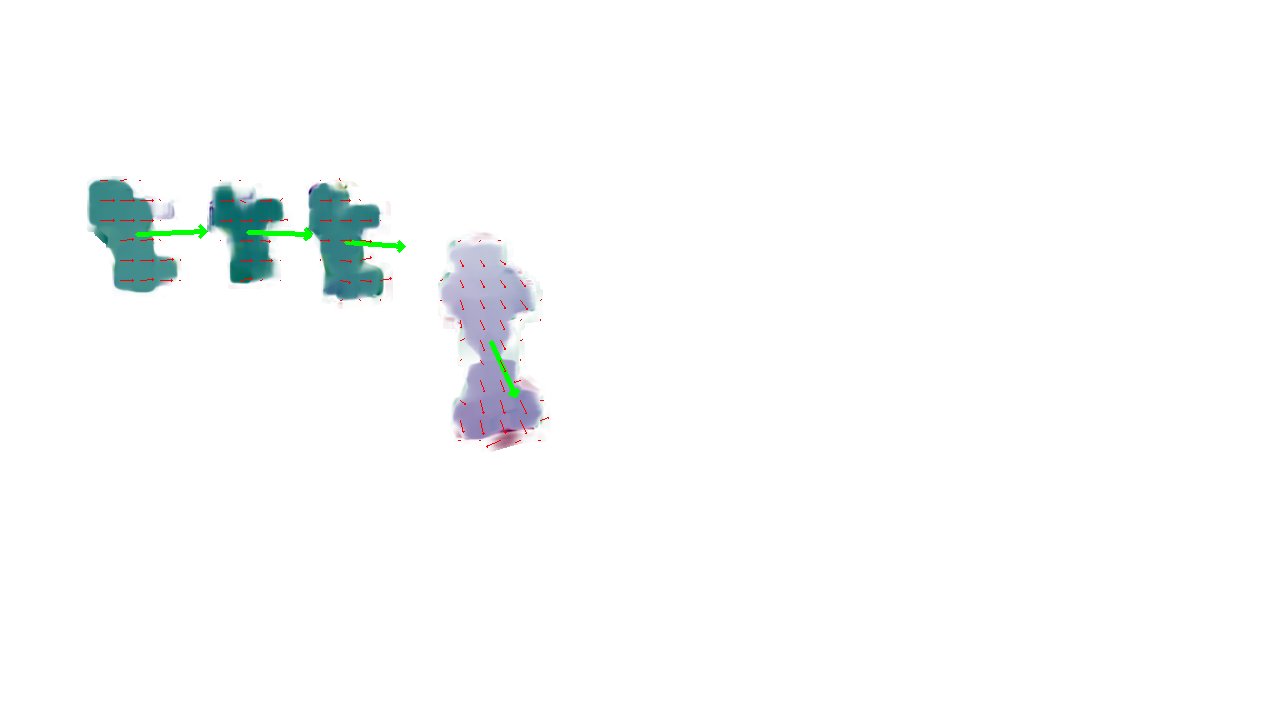
\includegraphics[width=0.6\textwidth]{figs/Pepper-optical-flow.png}
%     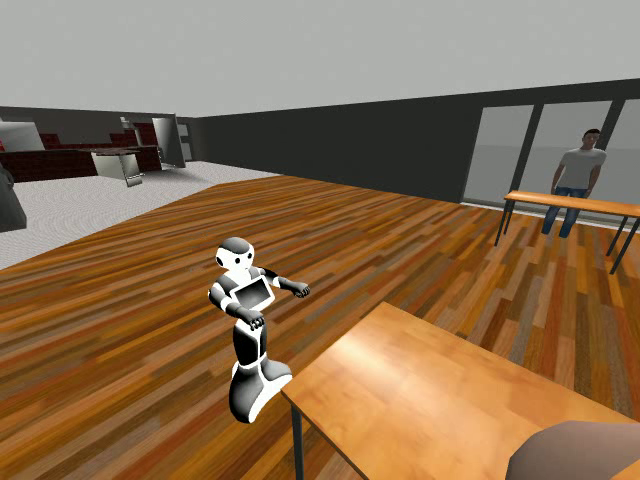
\includegraphics[width=0.4\textwidth]{figs/legibot-pepper-restaurant.png}
%     \caption{Sample Optical Flow}
%     \label{fig:enter-label}
% \end{figure}

\begin{figure}[ht]
  \centering
  \begin{subfigure}{0.5\textwidth}
    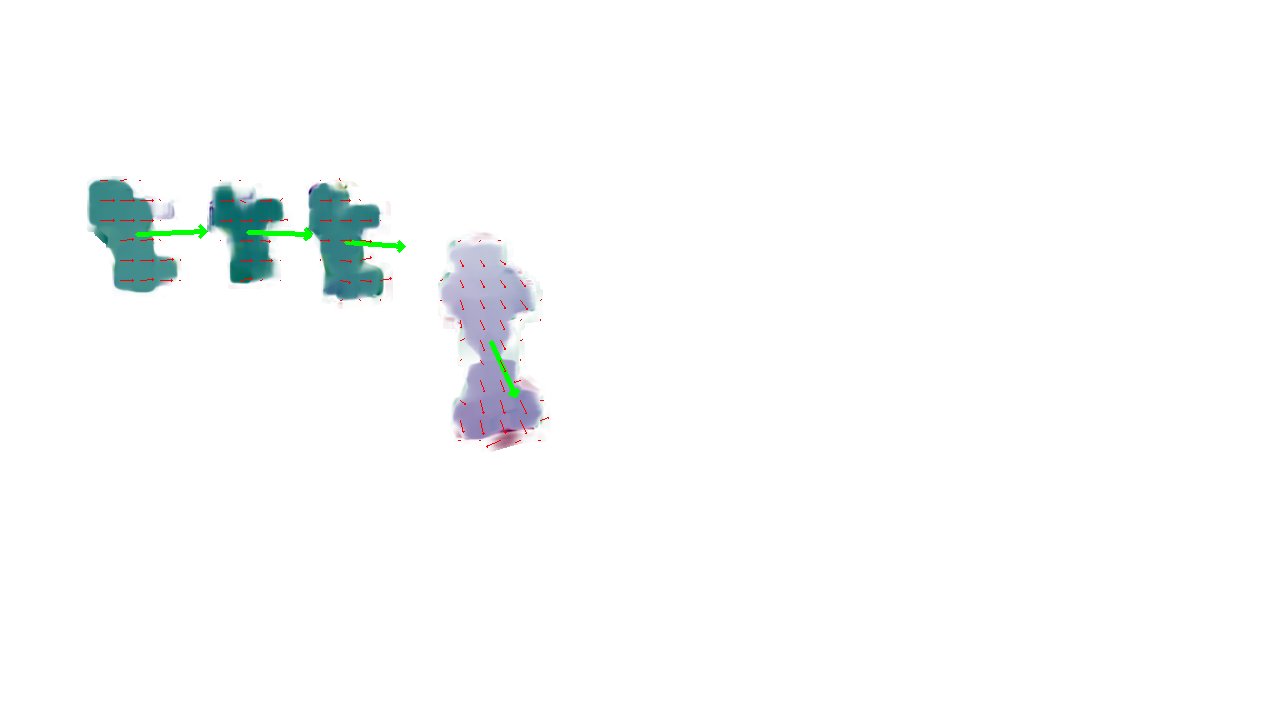
\includegraphics[width=\linewidth]{figs/Pepper-optical-flow.png}
    \caption{Sequence of Optical Flow outputs for the robot motion}
    \label{fig:sub1}
  \end{subfigure}
  \hspace{0.05\textwidth}
  \begin{subfigure}{0.35\textwidth}
    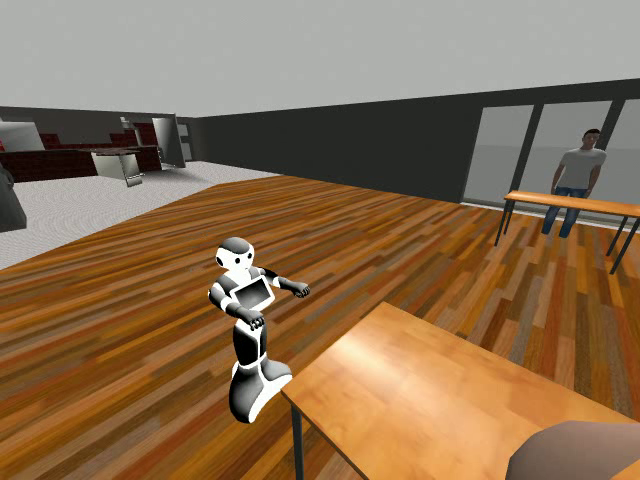
\includegraphics[width=\linewidth]{figs/legibot-pepper-restaurant.png}
    \caption{Normal View}
    \label{fig:sub2}
  \end{subfigure}
  \caption{Observer View}
  \label{fig:main}
\end{figure}

% Post-process
The process of calculating the optical flow image from the observer's perspective begins with capturing the frames as the observer. Optical flow algorithms analyze the pixel-level displacements between consecutive frames to estimate the apparent motion of objects within the scene. In the post-processing phase, we analyze the optical flow image to segment objects and distinguish the robot's motion. This segmentation and motion distinction process is essential ...

% \hl{See this:} \cite{park2023VRSickness} and \cite{gil2016estimating}

% \subsection{Focus of Expansion}

% The Focus of Expansion (FoE) $F_i$ in optical flow imagery refers to a specific point or region within the image where all optical flow vectors appear to converge. It is a concept used in computer vision and motion analysis to understand the motion of objects in a scene. 
% Theoretically, all we need are two vectors since we can simply take the lines defined by these two vectors and determine where they meet. This will be the focus of expansion. Of course, in reality, noise and other errors from the many steps to reach this point will result in imperfect optical flow vectors. Instead, the following formula considers a set of $n$ flow vectors \hl{$\{(v_i, u_i)\}$} from the detected object:

% \begin{equation}
% \begin{aligned}
% \mathfrak{F} & =\left(A^{T} A\right)^{-1} A^{T} \mathbf{b}
% \end{aligned}
% \end{equation}

% \noindent
% where
%     \begin{equation}
%     A=\left[\begin{array}{cc}
%     v_{0} & u_{0} \\
%     \cdots & \cdots \\
%     v_{n} & u_{n}
%     \end{array}\right] ,
%     \quad \mathbf{b}=\left[
%     \begin{array}{c}
%     b_{0} \\
%     \cdots \\
%     b_{n}
%     \end{array}\right]    
% \end{equation}

% \noindent
% and for each pixel $p_{i}=(x, y)$, 
% %the associated flow vector $\mathbf{v}=(u, v)$ gives $v_{i}=v, u_{i}=u$,  
% $b_{i}=x v-y u$.
% %
% \noindent
% It can finally be rewritten as:
% \begin{equation}
% \begin{aligned}
% \mathfrak{F} & =\
% \left[\begin{array}{c}
% \sum v_{i} b_{i} \sum u_{j}^{2}-\sum u_{i} b_{i} \sum v_{j} u_{j} \\
% -\sum v_{i} b_{i} \sum u_{j} v_{j}+\sum u_{i} b_{i} \sum u_{j}^{2}
% \end{array}\right]
% & -\frac{1}{\sum u_{j}^{2} v_{j}^{2}-\left(\sum v_{i} u_{i}\right)^{2}}
% \end{aligned}
% \end{equation}

% \noindent
% \textbf{TODO:} Move these equations to an appendix

% \begin{figure}
%     \centering
%     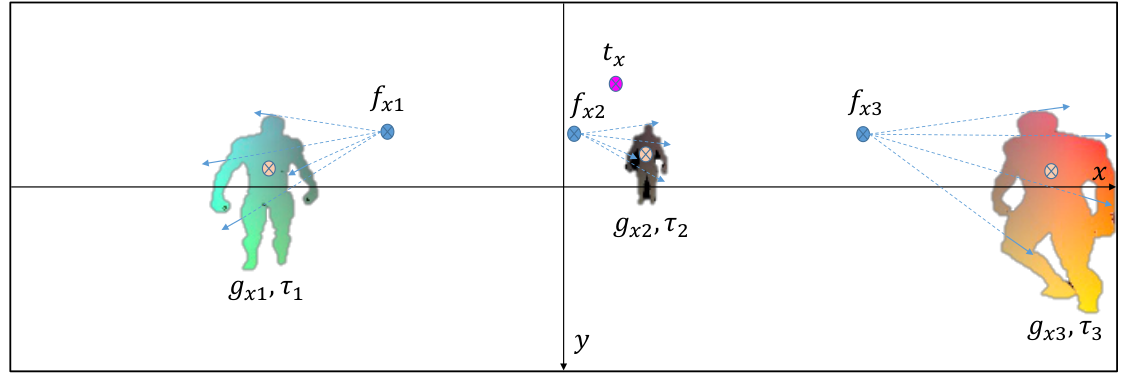
\includegraphics[width=0.5\textwidth]{figs/sample-FoE.png}
%     \caption{Focus of Expansion Example}
%     \label{fig:enter-label}
% \end{figure}

\subsection{Direction of Motion}
% The FoE does not always show where the robot is heading, for example when an object is approaching the observer, the motion lines would converge behind the moving object, and the FoE can be misleading. \\
% Then ...

% \hl{the image of this vector on the image plane is called the Focus of Expansion (FoE) when the camera moves forwards, or the Focus of Contraction (FoC) when it moves backward, see Fig. 1. Although FoE and FoC refer to opposite directions, their properties are very similar}

% \sethlcolor{cyan}
% \hl{
    Compute the DoM of the robot and calculate the difference between the direction of FoE vector and the robot-to-goal[i] direction.  This can be a metric to assess the legibility of the robot's motion w.r.t the potential goals in the environment.
% }
% \sethlcolor{yellow}





%\subsection{Context-aware Long-term Goal Prediction}

We propose to use a more sophisticated trajectory forecasting algorithm, that can make more realistic predictions, which in the end improve the overall result for the motion legibility.
%
We assume using a multi-modal prediction algorithm in Eq. (\ref{eq_dragan9}) that also takes into account the contextual cues $C$:

\begin{equation}
    \label{eq_P_G_with_context}
     P\left(G \mid \xi_{S \rightarrow \xi(t)}, C \right) 
\end{equation}

\noindent
Now, in order to improve the legibility of the robot motion, we can minimize the entropy of $G$:

\begin{equation}
    \label{eq_H_G}
    \min H(G) = -\mathbb{E} \left[\log P(G \mid \xi_{S \rightarrow \xi(t)}, C ) \right]
\end{equation}

We are inspired by the Inception Score in Generative Models literature, which propose to use a pre-trained neural network (the Inception Net [REF] trained on the
ImageNet [REF]) to ensure the generated samples are highly classifiable [REF]. Here, we are also interested in generating motions that are as classifiable as possible for the observers and in order to simulate the way an observer perceives and interpret the surrounding trajectories, we propose to use an independent prediction model that is trained on a dataset of motion trajectories.
We will discuss the potential bias of the proposed method in the Conclusion section [REF].

We decided to use the GoalGAN architecture [REF] to estimate \ref{eq_P_G_with_context}, which is trained on a relatively large dataset of long-term human trajectories. The model is in fact proposed to first estimate the goals.


\subsection{Using LLMs to Describe Potential Goals:}

Query: 



\begin{figure}[ht]
  \centering
  \begin{subfigure}{0.8\textwidth}
    \textbf{Query:} Given the robot's task of delivering dishes, along with the image and the characteristics of the environment, what could be the potential positions that the robot aims to reach?
    \vspace{10pt}
  \end{subfigure}

  \begin{subfigure}{\textwidth}
  \centering
    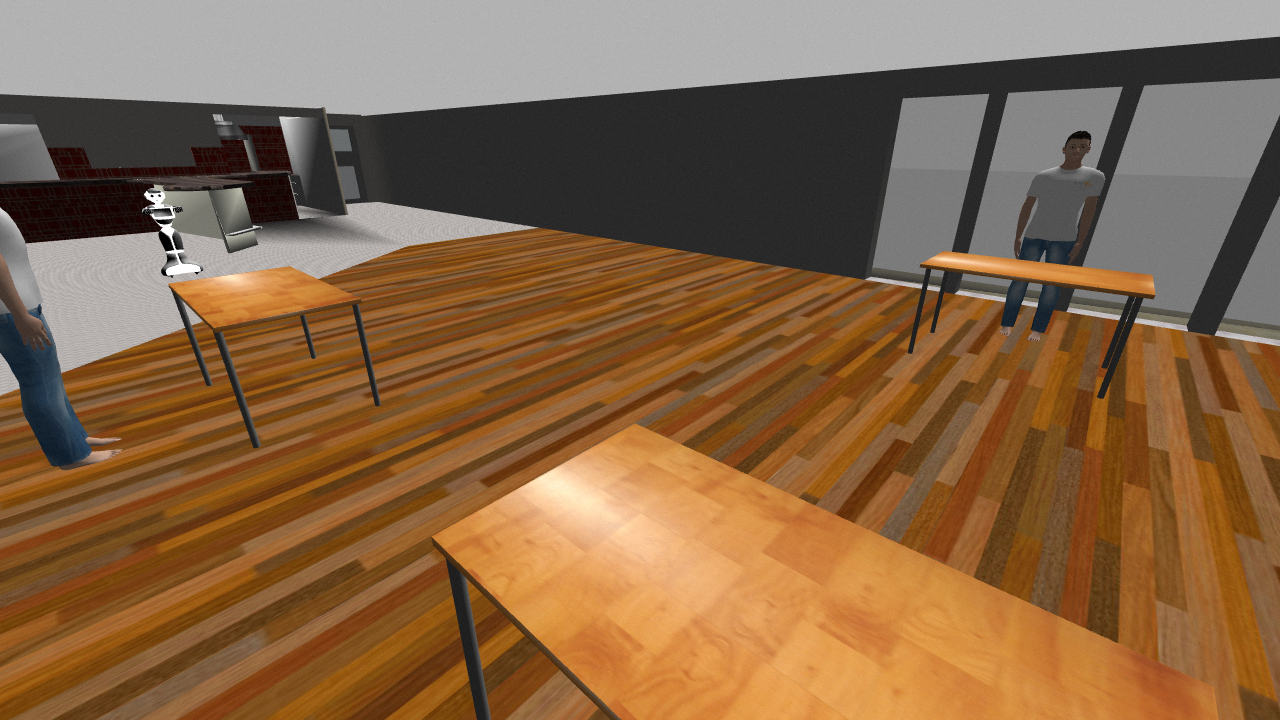
\includegraphics[width=0.8\linewidth]{figs/pepper-in-restaurant.png}
    \caption{Pepper Working in a Restaurant}
  \end{subfigure}

  \begin{subfigure}{\textwidth}
    \vspace{10pt}
    \textbf{Answer:} 
        The robot's potential goal positions for delivering dishes in the provided image are near the tables. Multiple tables around the room could serve as delivery points. Specifically: \\
        - The table closest to the robot and in front of the person wearing blue jeans could be a goal position. \\
        - The table on the far left, near the person standing by the window, is another potential goal position. \\
        - Any other visible tables in the room could also serve as goal positions based on the robot's needs.
  \end{subfigure}

  \caption{Asking AGI for Potential Goals of the Robot}
  \label{fig:vqa_example}
\end{figure}


\subsection{Synthesizing Legible Motions}
We need to modify the planner to become legibility-aware. This can happen by adding a gradient-descent-based process that iteratively updates the initial proposed trajectory to reach to the desired legibility score:


% \begin{figure}
%     \centering
%     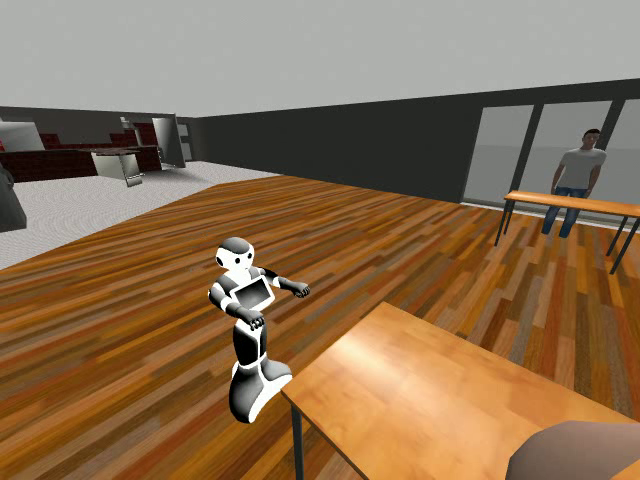
\includegraphics[width=0.6\textwidth]{figs/legibot-pepper-restaurant.png}

%     \caption{GoalGAN}
%     \label{fig:enter-label}
% \end{figure}




\section{Experimental Results}
\subsection{Simulation in Restaurant Setup}
One challenge with computing Optical Flow on simulated frames is that due to the lack of texture, it might become unstable during frames where there is zero or low level of motion in the scene. To fix this we have to preprocess the frames with a simple subtraction operator between the consecutive frames and estimate the total motion before passing the image to the optical-flow deep network.

\subsection{Why restaurants?}
\noindent
\hl{Todo:} to read the literature and review

In fact, robots have been already deployed in restaurants and thousands of them are in place. This type of situation usually contains a certain number of people: clients, waiters, ... . And the people are part of interaction scenarios with the robot(s). The clients might be new to this place and new to facing the robot in this restaurant, which means they wouldn't have a clear idea of the robot's behavior. 


% \begin{figure}
%     \centering
%     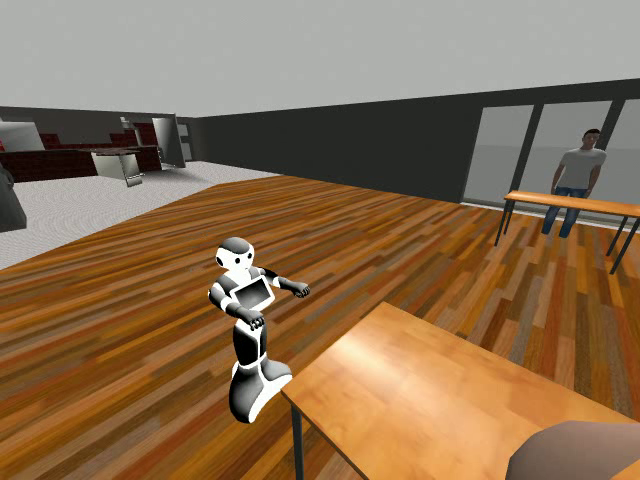
\includegraphics[width=0.4\textwidth]{figs/legibot-pepper-restaurant.png}
%     \caption{Pepper in Restaurant (Simulation)}
%     \label{fig:enter-label}
% \end{figure}

\subsection{Experiments with Real Robot}

% \begin{figure}
%     \centering
%     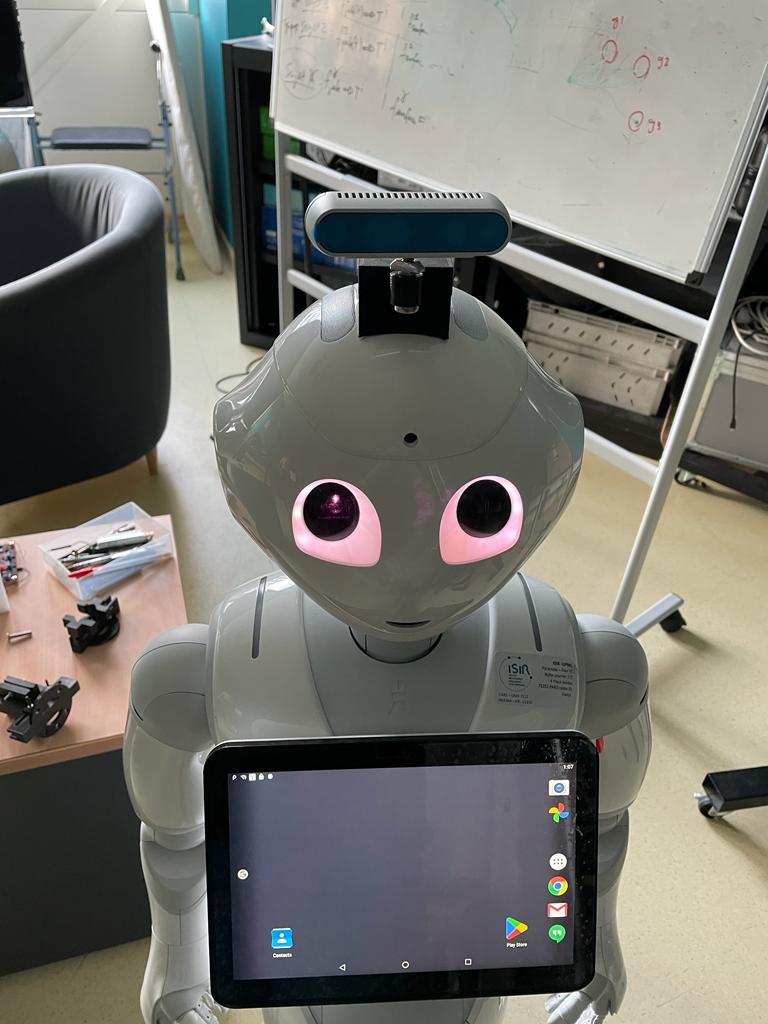
\includegraphics[width=0.3\textwidth]{figs/pepper-modified.jpeg}
%     \caption{Modified Pepper Robot}
%     \label{fig:enter-label}
% \end{figure}


\subsection{User Study}

\section{Conclusion}
\input{sections/conclusion}

%\section{References}

\begin{enumerate}
    \item Legibility and Predictability of Robot Motion
    \item Observer-Aware Legibility for Social Navigation
    \item Generating Legible Motion
    \item Viewpoint-Based Legibility Optimization
    \item A new approach to evaluating legibility: Comparing legibility frameworks using framework-independent robot motion trajectories
    \item A flexible optimization-based method for synthesizing intent-expressive robot arm motion
    \item A MIP-Based Approach for Multi-Robot Geometric Task-and-Motion Planning
    \item Wait Wait, Nonverbally Tell Me: Legibility for Use in Restaurant Navigation
%        \item
\end{enumerate}


%\bibliographystyle{IEEEtran}
\bibliographystyle{plain}
\bibliography{refs}

\end{document}


